\documentclass[beamer]{standalone}

\usepackage{tikz}

\usetikzlibrary{backgrounds}

\definecolor{almost-white}{HTML}{fefefe}

\begin{document}

\begin{standaloneframe}

\begin{tikzpicture}[
    grow=right,
    level 1/.style={
        sibling distance=2cm,
    },
    level 2/.style={
        sibling distance=1cm,
    },
    background rectangle/.style={ draw=almost-white, line width=0pt, },
    show background rectangle,
]

\node {\(U_n\)}
    child foreach \l in {1,2}
    { node {\(U_{\frac{n}{2}}\)}
        child foreach \l in {1,2}
        { node {} }
    }
    ;
\end{tikzpicture}
\end{standaloneframe}

\begin{standaloneframe}
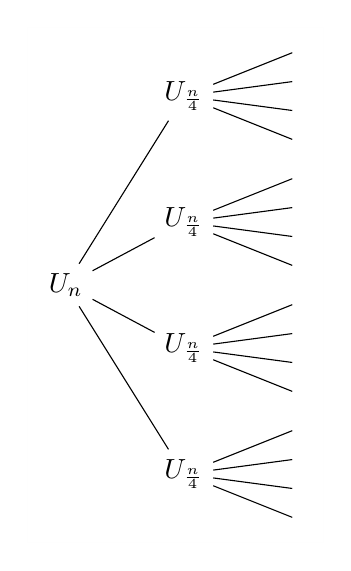
\begin{tikzpicture}[
    grow=right,
    level 1/.style={
        sibling distance=1.6cm,
    },
    level 2/.style={
        sibling distance=.4cm,
    },
    background rectangle/.style={ draw=almost-white, line width=0pt, },
    show background rectangle,
]

\node {\(U_n\)}
    child foreach \l in {1,2,3,4}
    { node {\(U_{\frac{n}{4}}\)}
        child foreach \l in {1,2,3,4}
        { node {} }
    }
    ;
\end{tikzpicture}

\end{standaloneframe}


\end{document}
